\documentclass[aspectratio=169]{beamer}
%% Remove draft for real article, put twocolumn for two columns
\usepackage[draft]{svmacro}
\usepackage[utf8]{inputenc}
\usepackage{verbatim}

%Information to be included in the title page:
\title{MATH 102: Ideas of Math}
\author{Day 15}
\date{Oct 17, 2023}

\begin{document}

\frame{\titlepage}

\begin{frame}
    \frametitle{ Exam Discussion }
    \begin{figure}
        \begin{center}
            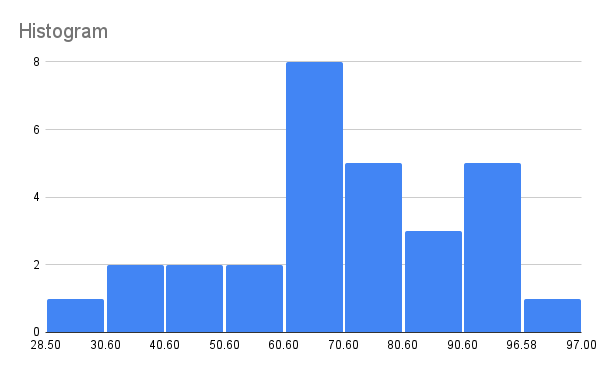
\includegraphics[width=0.7\textwidth]{Histogram-ideas.png}
        \end{center}
    \end{figure}
\end{frame}

\begin{frame}[fragile]
    \frametitle{ Power set }
    \begin{definition}
        Let $X$ be a set. The power set of $X$, written $\mathcal{P}()$ is the set of all subsets of $X$.

        Code:
        \begin{verbatim}
        \mathcal{P}(X)
        \end{verbatim}

    \end{definition}
\end{frame}

\begin{frame}
    Q: If $X$ has $n$ elements, how many elements does $\mathcal{P}(X)$ have?
\end{frame}
\end{document}
